%-------------------------------------------------------------------------------
%                            BAB III
%               		METODOLOGI PENELITIAN
%-------------------------------------------------------------------------------
% \fancyhf{} 
% \fancyfoot[R]{\thepage}
\chapter{METODE PENENILITIAN}

\par Dalam pengembangan model Long Short-Term Memory (LSTM), persiapan data yang tepat adalah langkah krusial yang dapat mempengaruhi kinerja model secara signifikan. Bab ini membahas berbagai teknik untuk mempersiapkan data numerik dan kategorikal, serta bagaimana menangani urutan dengan panjang yang bervariasi.

\section{Waktu dan Lokasi Penelitian}
Penelitian ini akan bertempat pada beberapa ruangan yang digunakan oleh mahasiswa Jurusan Informatika USK yang umumnya terletak pada lantai 3 blok A dan blok E Gedung Fakultas MIPA USK. Waktu yang dibutuhkan agar penelitian ini dapat di implementasikan adalah 4 bulan terhitung dari bulan Januari 2024 hingga Mei 2024.
\section{Jadwal Pelaksanaan Penelitian}

\section{Alat dan Bahan}
Alat dan Bahan yang akan digunakan pada penelitian ini terdiri dari beberapa perangkat keras (\textit{hardware}) dan perangkat lunak (\textit{software}) yang dijabarkan sebagai berikut:

\begin{enumerate}
\item Perangkat Keras
	\begin{itemize}
	\item Laptop Apple Macbook Air M1 2020 dengan RAM 8 \textit{Gigabyte}.
    \end{itemize}
\item Perangkat Lunak
	\begin{itemize}
	\item MacOS (18.1)
	\item Jupyter 
	\item Python 3.8.17
    \item NumPy (1.24.0)
    \item SQLite3 (3.39.4)
    \item Pandas (1.5.3)
    \item Joblib (1.2.0)
    \item scikit-learn (1.2.0)
    \item TensorFlow (2.11.0)
    \item Keras (2.11.0)
    \item Matplotlib (3.6.2)
    \item TensorFlow Keras Layers (2.11.0)
    \item itertools (built-in)
	\end{itemize}
\end{enumerate}

\section{Prosedur Penelitian}

%ISI 
\par Diagram Alir penelitian
\begin{center}
    \begin{figure}
        \centering
        \includegraphics[width=1\textwidth]{images/3-Diagram.drawio.pdf} 
        \caption{Diagram Alir Penelitian}
        \label{fig:3-diagram}
    \end{figure}
\end{center}
Prosedur penelitian ini dirancang untuk mensimulasikan spektrum atom dalam plasma pada kondisi kesetimbangan termal, dengan tujuan menentukan suhu eksitasi berdasarkan intensitas garis spektral. Pendekatan ini mengintegrasikan perhitungan kuantum mekanis, statistik termodinamika, dan pemodelan machine learning untuk analisis data spektral. Langkah-langkah simulasi diuraikan sebagai berikut:

\begin{itemize}
    \item \textbf{Desain Simulasi}
        \begin{itemize}
            \item \textbf{Perhitungan Tingkat Energi} \\
                  Tingkat energi atom dihitung menggunakan pendekatan kuantum mekanis. Persamaan Schrödinger digunakan untuk atom hidrogen, memberikan solusi analitik untuk energi \( E_n = -\frac{13.6}{n^2} \, \text{eV} \), dengan \( n \) sebagai bilangan kuantum utama \citep{Griffiths2005}. Untuk atom yang lebih kompleks, metode Hartree-Fock diterapkan untuk memperkirakan energi elektron dalam medan efektif multi-elektron, dengan memperhitungkan interaksi antar-elektron \citep{Szabo1996}. Data tingkat energi divalidasi terhadap basis data NIST \citep{NIST2025}.

            \item \textbf{Pemodelan Populasi Energi} \\
                  Populasi tingkat energi dimodelkan menggunakan distribusi Boltzmann, seperti pada Persamaan~\eqref{eq:boltzmann}:
                  \begin{equation}
                      N_i = \frac{N g_i e^{-\frac{E_i}{k_B T}}}{Z}, \label{eq:boltzmann}
                  \end{equation}
                  di mana \( N_i \) adalah populasi pada tingkat energi \( E_i \), \( g_i \) adalah degenerasi, \( k_B = 8.617 \times 10^{-5} \, \text{eV/K} \), \( T \) adalah suhu, dan \( Z = \sum_i g_i e^{-\frac{E_i}{k_B T}} \) adalah fungsi partisi. Untuk plasma yang tidak sepenuhnya dalam kesetimbangan termal, persamaan Saha digunakan untuk memperkirakan distribusi ionisasi berdasarkan densitas elektron dan suhu \citep{Draine2011}. Parameter seperti \( g_i \) dan \( E_i \) diambil dari data NIST.

            \item \textbf{Pemodelan Profil Garis} \\
                  Spektrum dihasilkan dengan menginisialisasi rentang panjang gelombang (\( \lambda \)) dan menghitung intensitas untuk setiap transisi. Data tingkat energi dan degenerasi diambil dari basis data NIST \citep{NIST2025}. Intensitas garis spektral dihitung menggunakan:
                  \begin{equation}
                      I_{ij} = \frac{N g_i A_{ij} h \nu_{ij} e^{-\frac{E_i}{k_B T}}}{4\pi Z}, \label{eq:intensity_full}
                  \end{equation}
                  dengan \( h \nu_{ij} = \frac{h c}{\lambda_{ij}} \), \( h c \approx 1239.84 \, \text{eV·nm} \), dan \( A_{ij} \) sebagai koefisien Einstein untuk emisi spontan \citep{rybicki-1985}. Profil garis dimodelkan menggunakan distribusi Gaussian untuk memperhitungkan efek pelebaran Doppler dan tekanan, menghasilkan panjang gelombang dan intensitas yang dinormalisasi.

            \item \textbf{Parameter Plasma} \\
                  Simulasi menggunakan suhu plasma \( T = 10.000 \, \text{K} \) dan densitas elektron tipikal untuk plasma astrofisika (\( n_e \approx 10^{12} \, \text{cm}^{-3} \)) \citep{Draine2011}. Parameter ini dipilih untuk mencerminkan kondisi kesetimbangan termal lokal (LTE) yang relevan dengan analisis spektral.

            \item \textbf{Data dan Sumber} \\
                  Data utama berasal dari basis data NIST untuk tingkat energi, degenerasi, dan koefisien Einstein \citep{NIST2025}. Literatur tambahan, seperti \citet{rybicki-1985} dan \citet{Draine2011}, digunakan untuk validasi model dan parameter plasma.

            \item \textbf{Validasi Model Simulasi} \\
                  Hasil simulasi divalidasi dengan membandingkan panjang gelombang dan intensitas garis spektral dengan data eksperimen dari NIST \citep{NIST2025}. Deviasi dianalisis untuk memastikan akurasi model dalam memprediksi suhu eksitasi.

            \item \textbf{Pengumpulan Data} \\
                  Data spektral dikumpulkan dari simulasi dan disimpan dalam format numerik untuk analisis lebih lanjut. Data ini mencakup panjang gelombang, intensitas, dan parameter transisi untuk setiap garis spektral.
        \end{itemize}

    \item \textbf{Normalisasi Data} \\
          Untuk memastikan konsistensi dalam analisis, intensitas spektral dinormalisasi menggunakan rumus:
          \begin{equation}
              I' = \frac{I - I_{\min}}{I_{\max} - I_{\min}}, \label{eq:normalization}
          \end{equation}
          di mana \( I' \) adalah intensitas yang dinormalisasi, \( I \) adalah intensitas asli, serta \( I_{\min} \) dan \( I_{\max} \) adalah nilai minimum dan maksimum dari dataset. Normalisasi ini memfasilitasi perbandingan antar garis spektral dan persiapan data untuk pemodelan machine learning.

    \item \textbf{Perancangan Model Transformer} \\
          Model Transformer dirancang untuk menganalisis pola dalam data spektral, dengan arsitektur berdasarkan mekanisme perhatian (attention mechanism) \citep{Vaswani2017}. Pelatihan dilakukan menggunakan dataset spektral yang dinormalisasi, dengan optimasi parameter untuk memprediksi suhu plasma atau karakteristik spektral lainnya. Detail pelatihan mencakup penggunaan fungsi kerugian entropi silang dan optimizer Adam.

    \item \textbf{Persiapan Data untuk Model LSTM}
        \begin{itemize}
            \item \textbf{Arsitektur LSTM} \\
                  Model Long Short-Term Memory (LSTM) digunakan untuk analisis sekuensial data spektral, memanfaatkan kemampuan memori jangka panjang \citep{brownlee2017}. Arsitektur ini divisualisasikan pada Gambar~\ref{fig:lstm_architecture}.
                  \begin{figure}[h]
                      \centering
                      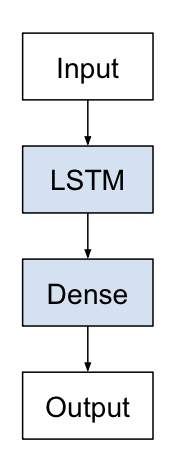
\includegraphics[width=0.2\textwidth]{images/lstm1.png}
                      \caption{Arsitektur LSTM untuk analisis data spektral \parencite{brownlee2017}.}
                      \label{fig:lstm_architecture}
                  \end{figure}

            \item \textbf{Persiapan Data Numerik} \\
                  Data numerik, seperti intensitas dan panjang gelombang, dinormalisasi untuk mempercepat pelatihan dan meningkatkan konvergensi model LSTM. Metode yang digunakan adalah Min-Max Scaling, sesuai dengan Persamaan~\eqref{eq:normalization}, dan Z-score Normalization untuk distribusi data yang lebih simetris \parencite{brownlee2017}.

            \item \textbf{Persiapan Data Kategorikal} \\
                  Data kategorikal, seperti jenis transisi atau spesies atom, diubah menjadi format numerik menggunakan One-Hot Encoding atau Label Encoding. One-Hot Encoding menghasilkan vektor biner untuk setiap kategori, sedangkan Label Encoding menetapkan nilai integer unik \parencite{brownlee2017}.

            \item \textbf{One-Hot Encoding} \\
                  One-Hot Encoding diimplementasikan menggunakan pustaka scikit-learn, seperti ditunjukkan pada Listing~\ref{lst:one_hot_encoding}:
                  \begin{lstlisting}[language=Python, caption=Contoh One-Hot Encoding dengan scikit-learn, label=lst:one_hot_encoding]
from sklearn.preprocessing import OneHotEncoder
encoder = OneHotEncoder()
encoded_data = encoder.fit_transform(data).toarray()
                  \end{lstlisting}
        \end{itemize}
\end{itemize}

\begin{theorem}
Ini adalah sebuah teorema.
\end{theorem}

\begin{definition}
Ini adalah definisi.
\end{definition}

\begin{remark}
Ini adalah catatan tanpa nomor.
\end{remark} 

\begin{proof}
Ini adalah bukti.
\end{proof}
 \begin{example}
        f
 \end{example}


 \begin{table}[H]
    \centering
    \caption{Perbandingahn  LIBS}
    \label{tab:performa_ml}
    \centering
    \begin{tabular}{lcccc}
      \toprule
      Model & Akurasi (\%) & Presisi (\%) & Recall (\%) & RMSE \\
      \midrule
      Random Forest & 95.2 & 94.8 & 95.1 & 0.12 \\
      SVM & 89.7 & 88.5 & 90.2 & 0.21 \\
      Transformer & 97.1 & 96.9 & 97.0 & 0.08 \\
      \midrule
      CNN & 93.4 & 92.7 & 93.5 & 0.15 \\
      \bottomrule
    \end{tabular}
    
    \smallskip
    \footnotesize
    \textit{Keterangan:} Data diperoleh dari 100 sampel logam dengan 5 kelas komposisi.
  \end{table}

% Baris ini digunakan untuk membantu dalam melakukan sitasi
% Karena diapit dengan comment, maka baris ini akan diabaikan
% oleh compiler LaTeX.
%\begin{comment}
%\bibliography{daftar-pustaka}
%\end{comment}